\documentclass{article}
\usepackage{PRIMEarxiv}
\usepackage{picins}
\usepackage[UTF8]{ctex}
\usepackage[utf8]{inputenc} % allow utf-8 input
\usepackage[T1]{fontenc}    % use 8-bit T1 fonts
\usepackage{hyperref}       % hyperlinks
\usepackage{url}            % simple URL typesetting
\usepackage{booktabs}       % professional-quality tables
\usepackage{amsfonts}       % blackboard math symbols
\usepackage{nicefrac}       % compact symbols for 1/2, etc.
\usepackage{microtype}      % microtypography
\usepackage{lipsum}
\usepackage{fancyhdr}       % header
\usepackage{graphicx}       % graphics
\graphicspath{{media/}}     % organize your images and other figures under media/ folder
\usepackage{enumerate}
\setlength{\parindent}{2em}

\begin{document}
\pagestyle{empty}
\noindent
\begin{minipage}[t]{0.45\linewidth}
	\noindent\parpic{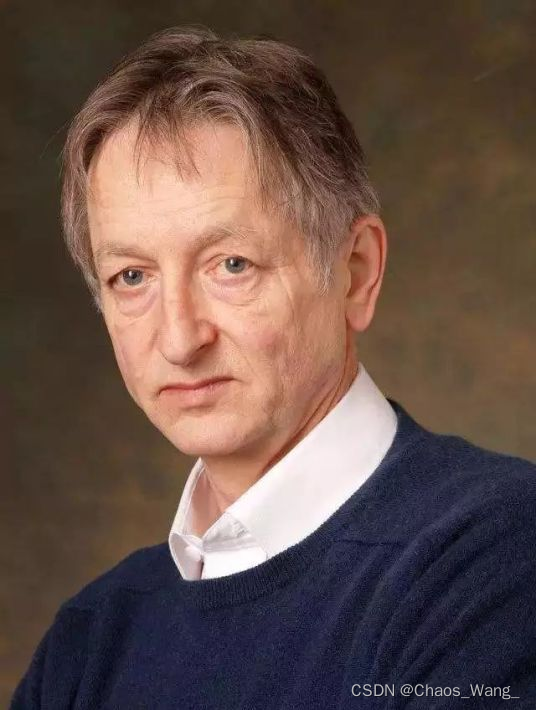
\includegraphics[height=1.5in,width=1in,clip,keepaspectratio]{Hinton.png}}
	\noindent{\bf Hinton} is a pioneer in artificial intelligence and deep learning, known as the "Father of Deep Learning." He promoted the backpropagation algorithm and proposed the Deep Belief Network (DBN) in 2006, leading to the resurgence of deep learning. His team developed the famous AlexNet, which marked the widespread application of deep learning in computer vision. As a professor at the University of Toronto and a researcher at Google Brain, Hinton has had a profound impact on deep learning optimization and model development. Together with Yann LeCun and Yoshua Bengio, he is known as one of the "Three Giants of Deep Learning" and received the Turing Award in 2018.
\end{minipage}
\hfill
\begin{minipage}[t]{0.45\linewidth}
	\noindent\parpic{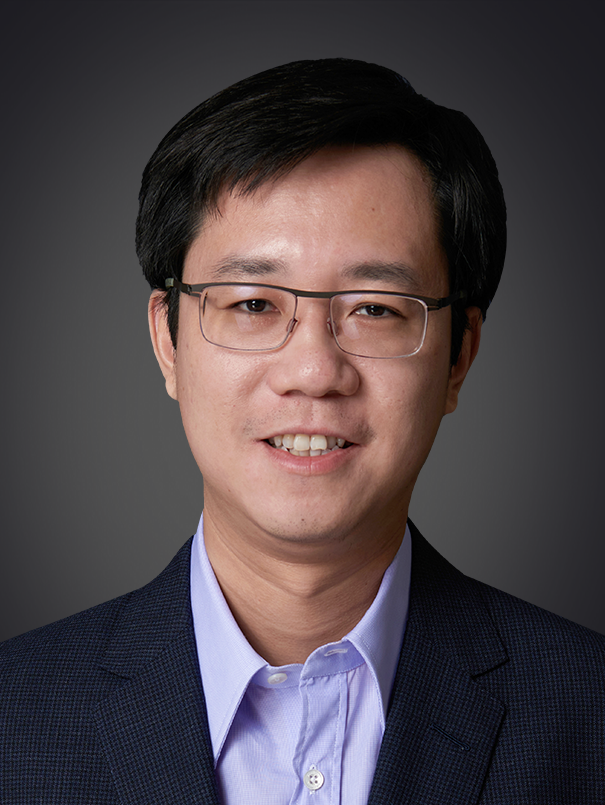
\includegraphics[height=1.5in,width=1in,clip,keepaspectratio]{Kaiming-He.png}}
	\noindent{\bf Kaiming-He} is a renowned researcher in computer vision and currently the Chief Scientist at Meta AI. Previously, he was a researcher at Microsoft Research. He proposed ResNet (Residual Network), which achieved groundbreaking results in the 2015 ImageNet competition, significantly advancing the application of deep learning in the field of vision. His research spans multiple areas, including deep learning architectures and object detection, making him a leading figure in artificial intelligence.
\end{minipage}

\vspace{2cm} % Insert 2 centimeter of vertical space.

\noindent
\begin{minipage}[t]{0.45\linewidth}
	\par\noindent 
	\parbox[t]{\linewidth}{
		\noindent\parpic{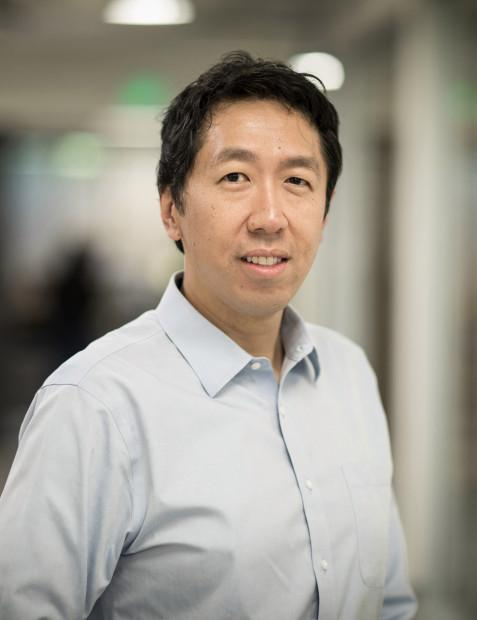
\includegraphics[height=1.5in,width=1in,clip,keepaspectratio]{Andrew.jpg}}
		\noindent{\bf Andrew Ng} is a renowned scholar and educator in the field of artificial intelligence and machine learning. He is a former professor at Stanford University, a co-founder of the Google Brain project, and the former Chief Scientist at Baidu. He is dedicated to promoting the adoption and application of AI, having founded the online education platform Coursera and offering a highly popular machine learning course, making significant contributions to global AI education and technology development.}
\end{minipage}
\hfill
\begin{minipage}[t]{0.45\linewidth}
	\parbox[t]{\linewidth}{
		\noindent\parpic{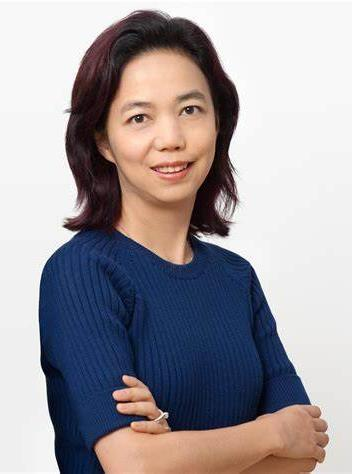
\includegraphics[height=1.5in,width=1in,clip,keepaspectratio]{FeiFei-Li.jpg}}
		\noindent{\bf FeiFei-Li} is a distinguished scientist in the field of computer vision and a professor of computer science at Stanford University. She previously served as the Chief Scientist of AI and Machine Learning at Google Cloud. She founded the ImageNet project, which revolutionized deep learning in computer vision. Her research spans areas such as visual understanding and AI ethics, contributing significantly to both the technological advancement and societal impact of AI.}
\end{minipage}

\end{document}
